\documentclass[slidestop,compress,mathserif, xcolor=table]{beamer}
\usetheme{Madrid}
\setbeamertemplate{headline}{}
\definecolor{scigreen}{RGB}{70,116,60}
\setbeamercolor{structure}{fg=scigreen}
\setbeamercovered{highly dynamic}

\usepackage[T1]{fontenc}
\usepackage{lmodern}
\usepackage[utf8]{inputenc}
\usepackage[english]{babel}
\usepackage{graphicx}
\usepackage{amsmath}
\usepackage{amssymb}
\usepackage{listings}

\title{Improving Rasterific}
\author[Chi, William]{Chi, William}
\institute[DIKU]{Department of Computer Science, University of Copenhagen}
\date{\today}

\begin{document}

\frame{\titlepage}
\begin{frame}[c]{Project}
    \begin{itemize}
    \item Briefly describe
    \item what this project is about
    \end{itemize}
\begin{figure}
\centering
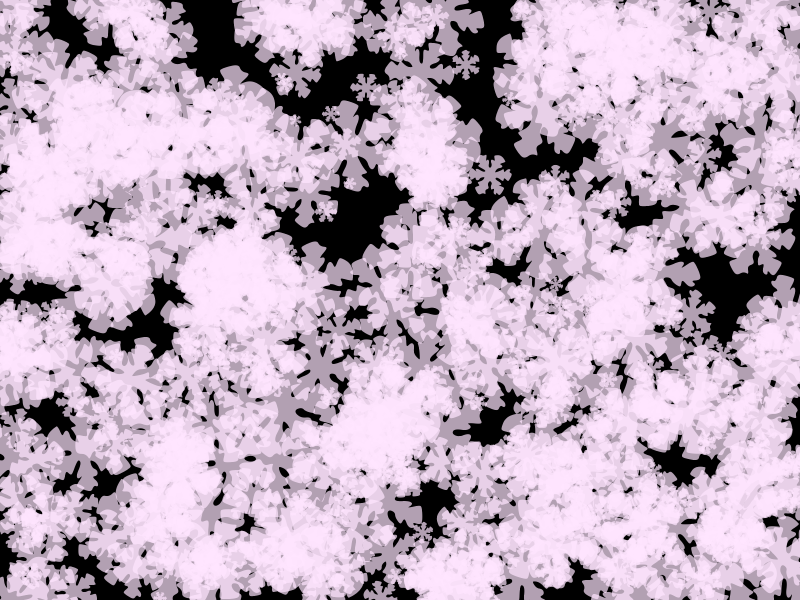
\includegraphics[width=0.3\linewidth]{../flakes}

\includegraphics[width=0.3\linewidth]{../bigsquare}
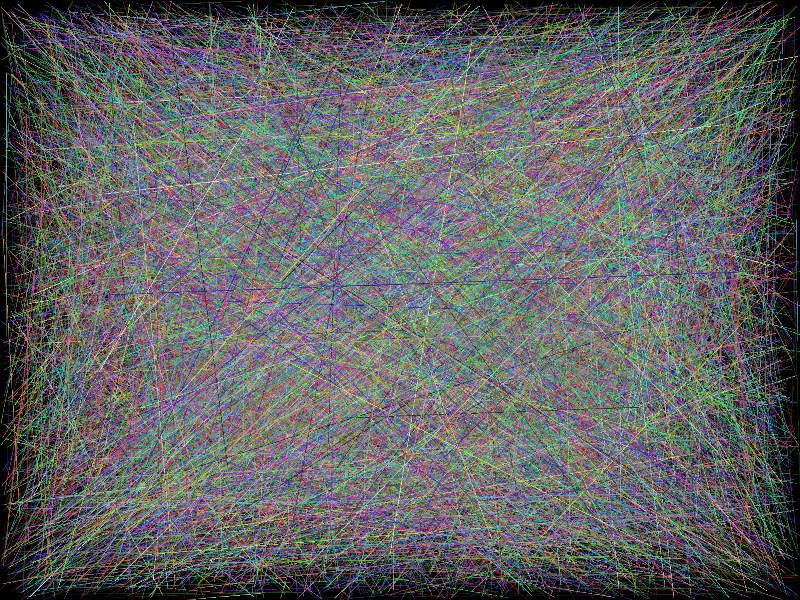
\includegraphics[width=0.3\linewidth]{../lines}
\end{figure}
\end{frame}

\begin{frame}[c]{Rasterific}
  \begin{itemize}
  \item An open source vector graphics rasterizer.
  \item Written in Haskell.
  \item No parallelism.
  \end{itemize}

\begin{figure}[h!]
  \centering
  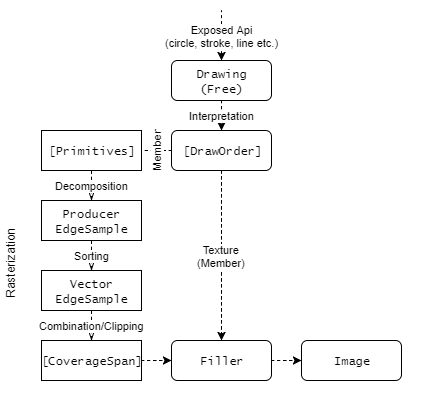
\includegraphics[width=.4\linewidth]{../rasterific-pipeline}
  \caption{Approximation of the Rasterific pipeline.}
\end{figure}

\end{frame}

\begin{frame}[c]{Experiments}
  \begin{itemize}
  \item bla
  \item bla
  \item bla
  \end{itemize}

  \begin{figure}[H]
  \centering
  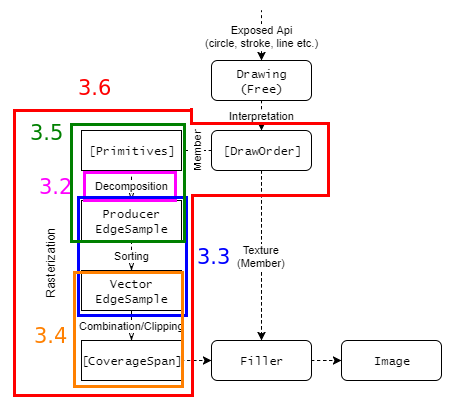
\includegraphics[width=.4\linewidth]{../rasterific-pipeline-flot}
  \caption{Parallelisation granularity in the Rasterific pipeline.}
  \label{fig:rasterific-pipeline-flot}
\end{figure}
\end{frame}

\begin{frame}

  
    overview of experiments - use same pipeline picture, annotated (on the same position in the slide for maximum goodness)

I have an idea for a tree-like picture - TBA

\end{frame}
\begin{frame}[c]{Decomposition of \texttt{Primitives}}
  \begin{itemize}
  \item Fine grained parallelism.
  \item Simple divide-and-conquer -- straightforward implementaion.
  \end{itemize}
  \begin{figure}[h!]
    \centering
    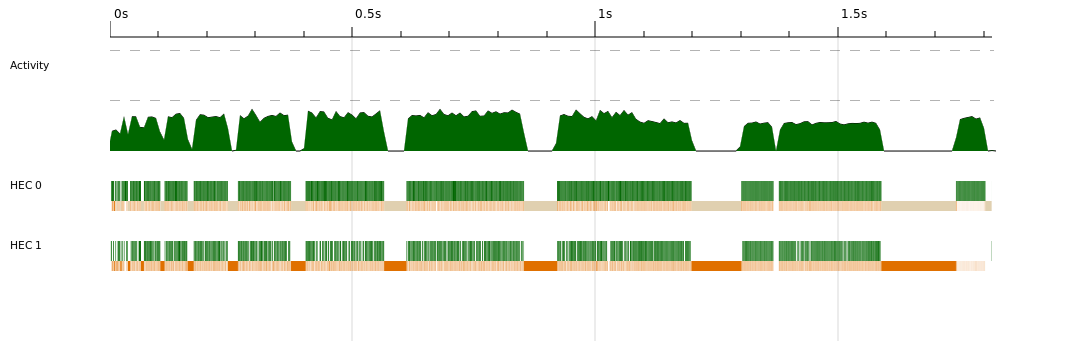
\includegraphics[width=0.75\linewidth]{../threadscope/lines/single-line-every-10}
    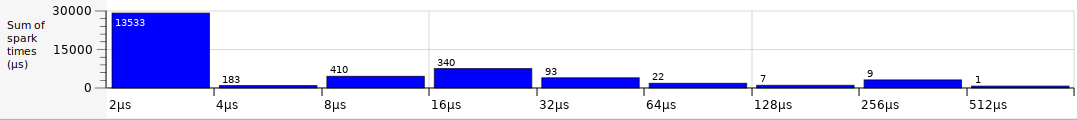
\includegraphics[width=0.4\linewidth]{../threadscope/lines/single-line-every-10-spark-times}
    \caption{ThreadScope output for decomposing a 1M px long line.}
  \label{fig:line-thread-sparks}

\end{figure}
\end{frame}
% NOTE: each experiment slide should be fairly brief during presentation -- not too many technical details, rather an explanation of parallel granularity + what we saw in threadscope
\begin{frame}[c]{Sorting \texttt{EdgeSamples}}
  \begin{itemize}
  \item Courser grained parallelism.
  \item Complex implementation.
  \end{itemize}
 \begin{figure}[h!]
  \centering
  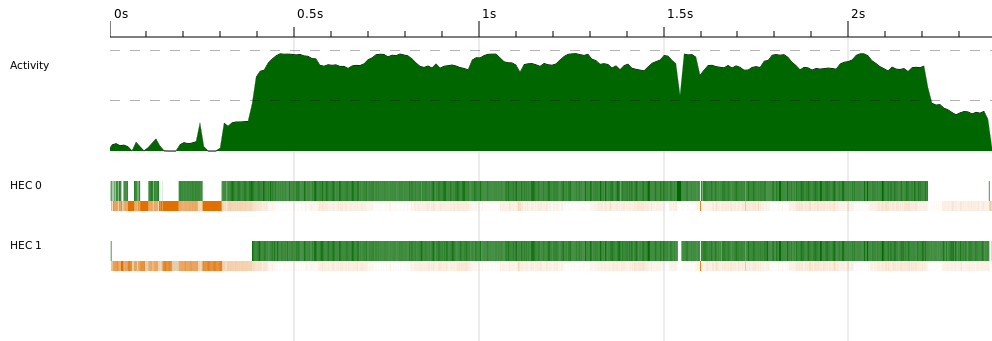
\includegraphics[width=0.6\linewidth,trim={4cm 2cm 0 0},clip]{../threadscope/sorting/sorting-final}
  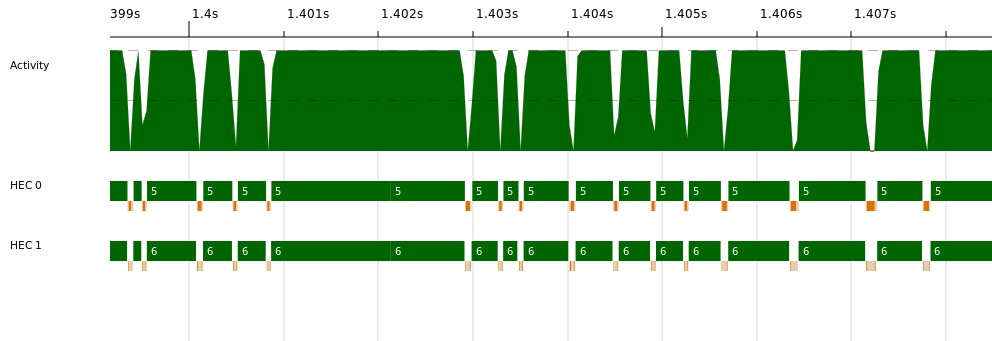
\includegraphics[width=0.3\linewidth,trim={8cm 2cm 5cm 0},clip]{../threadscope/sorting/sorting-final-zoom}
  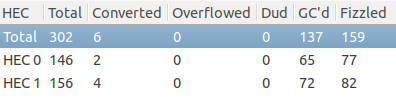
\includegraphics[width=0.25\linewidth]{../threadscope/sorting/sorting-final-sparks}
  \caption{ThreadScope output for sorting 1.000.000 \texttt{EdgeSample}s.}
  \label{fig:sorting-thread}
\end{figure}

\end{frame}

\begin{frame}[c]{Combining \texttt{EdgeSamples}}
description + threadscope
\end{frame}

\begin{frame}[c]{Filling \texttt{DrawOrders}}
description + threadscope
\end{frame}

\begin{frame}[c]{Benchmarks and Results}
maybe some graphical representation of the table from the report
\end{frame}

\begin{frame}[c]{Evaluation}
Why we got these results
\end{frame}

\begin{frame}[c]{Further Work and Conclusion}
\end{frame}
\end{document}